\chapter{Time Plan}
\label{ch:timeline}

\begin{table}[H]
\small
\setlength{\tabcolsep}{8pt}
\renewcommand{\arraystretch}{1.5}
\centering
\caption{Actual Project Development Phases and Objectives}
\label{tab:project_phases}
\begin{tabularx}{\textwidth}{@{}p{0.28\textwidth} X@{}}
\toprule
\textbf{Phase and Duration} & \textbf{Main Objectives} \\
\midrule

\textbf{Phase 1 (10.15--10.31): Foundation Setup and Project Onboarding} &
Complete checklist and ethics forms; define initial research directions for virtual try-on, recommendation LLMs, and outfit logic; deploy and validate project website. \\

\textbf{Phase 2 (11.01--11.14): Literature Review and Technical Research} &
Survey try-on frameworks (e.g., Qwen-Image-Edit, diffusion-based methods); evaluate LLM candidates (Qwen3-VL); collect baseline performance references. \\

\textbf{Phase 3 (11.15--12.03): System Modeling and Prototype Design} &
Draft UML diagrams; refine functional requirements; develop mid-fidelity UI prototypes; align personas and user stories with SRS. \\

\textbf{Phase 4 (12.04--12.21): Interim Report} &
Integrate research findings; refine system architecture; update use-case coverage and requirements traceability for submission. \\

\textbf{Phase X (12.22--01.13): Final Exams Review} &
\textit{(No project objectives required; academic preparation period.)} \\

\textbf{Phase 5 (01.14--01.31): Frontend Development and Login Integration} &
Implement frontend interfaces and complete login module integration; establish initial frontend-backend interaction and ensure basic user authentication workflow. \\

\textbf{Phase 6 (02.01--02.15): Backend Development and Initial Integration} &
Design backend architecture and database schema; implement partial recommendation AI functionality; achieve initial frontend-backend integration for the “My Wardrobe” module. \\

\textbf{Phase 7 (02.16--02.29): Calendar Module Integration and External API Integration} &
Complete initial frontend-backend integration for the “My Calendar” module; successfully integrate weather API to support context-aware features. \\

\textbf{Phase 8 (03.01--03.14): System Integration and Feature Enhancement} &
Complete frontend-backend integration for wardrobe analysis; replace manual tagging with LLM-based automatic tagging in the wardrobe module; integrate recommendation module, though outputs remained unstructured at this stage. \\

\textbf{Phase 9 (03.15--03.31): Final Optimization and Testing} &
Refine overall UI and visual consistency; improve recommendation module to produce structured outputs; complete virtual try-on pipeline; conduct system testing and questionnaire-based user evaluation. \\

\bottomrule
\end{tabularx}
\end{table}

As shown in Table \ref{tab:project_phases}, in the first semester we mainly focused on research and report writing, while in the second semester we focused on system implementation and integration. 

During the development process, the work related to databases and models is basically carried out in parallel, while the internal functions of each module are gradually expanded in stages (e.g. We implemented the wardrobe module first, and then expanded to wardrobe analysis). Overall, we first completed the development of the frontend and login functions, followed by the construction of the backend and database. Based on this, we gradually integrated modules such as wardrobe management, calendar, analysis, recommendation, and virtual try on into the system.\\

\begin{figure}[H]
    \centering
    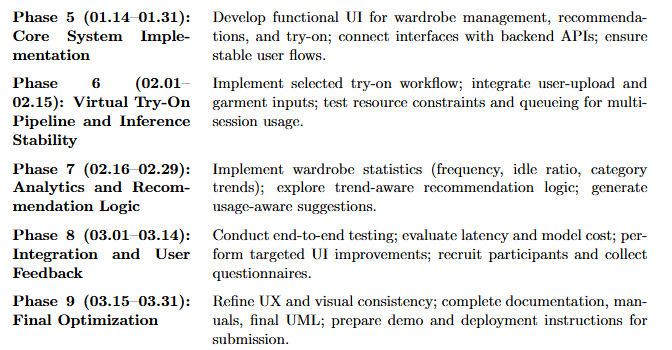
\includegraphics[width=0.8\textwidth]{images/Section8/original.png}
    \\[0.5cm]
    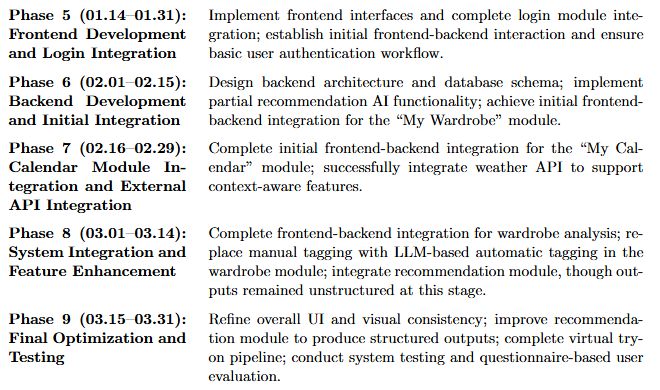
\includegraphics[width=0.8\textwidth]{images/Section8/actual.png}
    \caption{Original plan (top) and Actual plan (bottom)}
    \label{fig:plan_compare}
\end{figure}

Figure~\ref{fig:plan_compare} compares the original schedule set at the beginning of the project with the final execution schedule. It can be seen that in the bottom one, each module is gradually stacked and pushed forward. Due to insufficient familiarity with model deployment and integration, the overall development progress of related modules is slower than that of database based functional development. In contrast, the original schedule had a vague overall arrangement due to a lack of in-depth understanding of the project.

\begin{figure}[H]
    \centering
    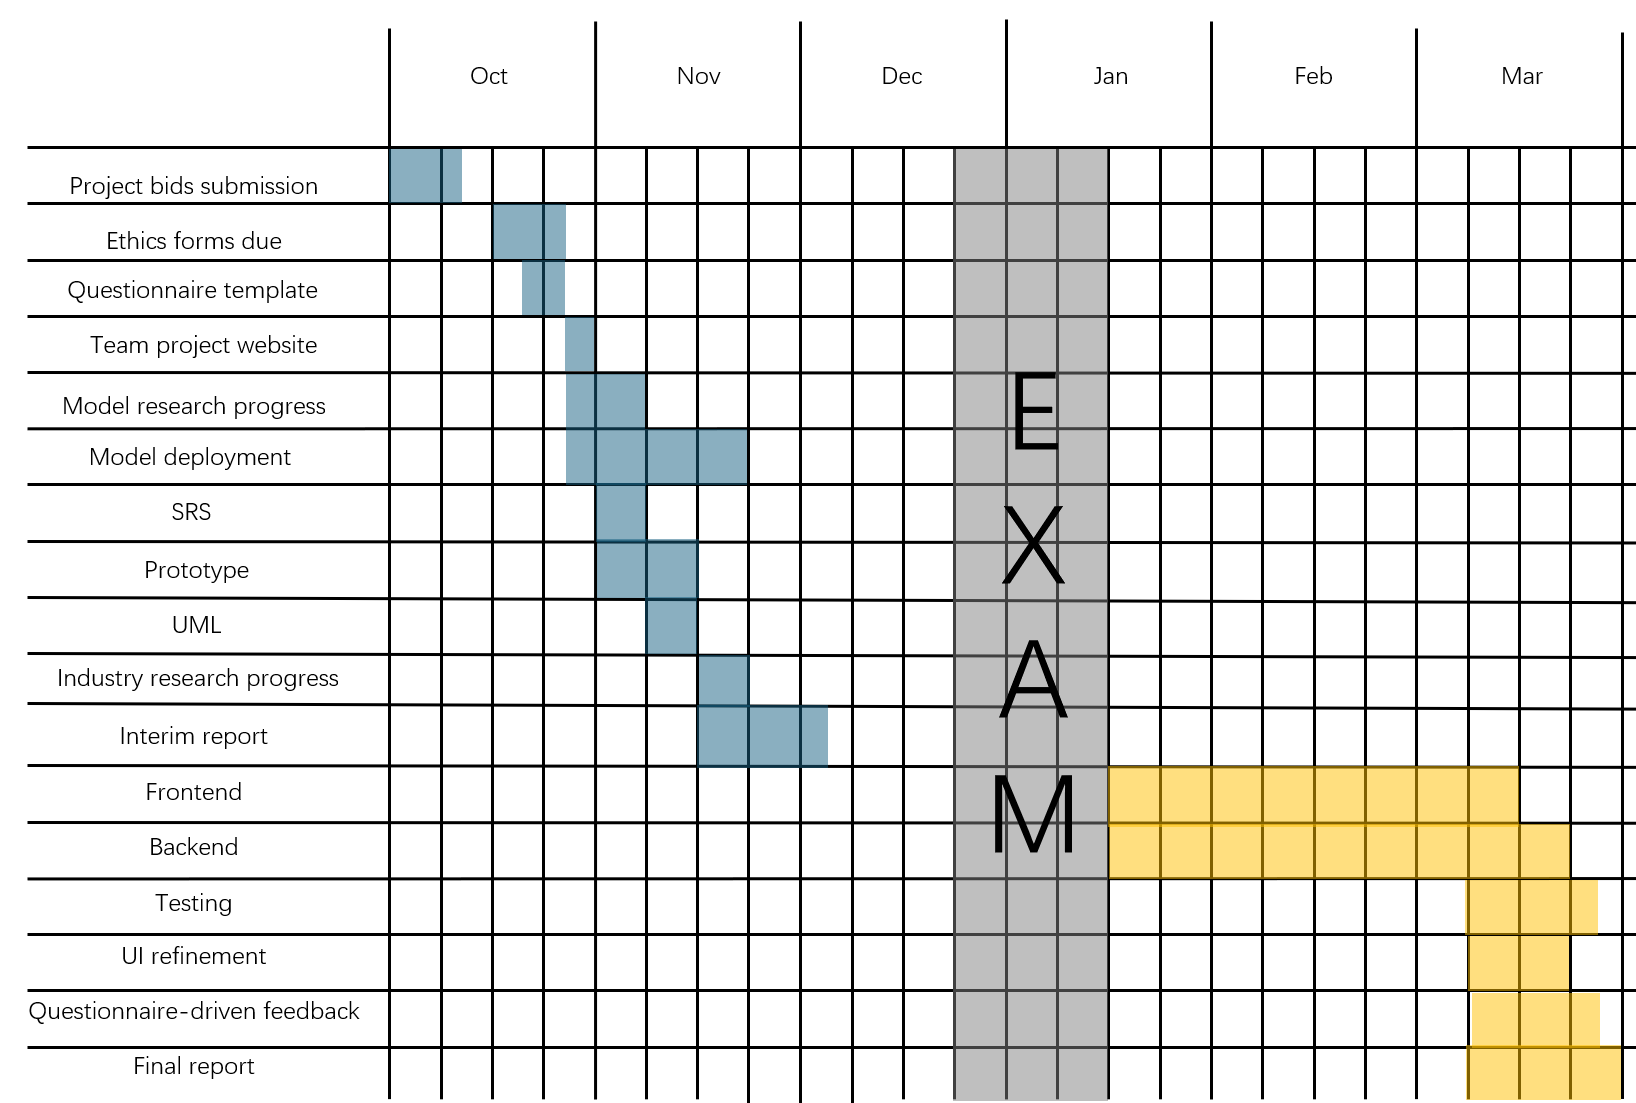
\includegraphics[width=1.0\textwidth]{images/Section8/gantt.png}
    \caption{Gantt chart}
\end{figure}

This Gantt chart highlights three key characteristics of the project schedule:
\begin{itemize}
    \item We conducted research before the winter holiday, establishing a stable foundation for implementation.
    \item Development is concentrated after the exam period, with front-end, back-end, and integration as the main workload.
    \item In the final stage, we focused on testing, UI optimization, and questionnaire-based evaluation to validate the system and improve user experience.
\end{itemize}

Overall, although there were some differences between the actual development sequence and the initial plan, the adjusted timeline allowed us to prioritize the core functions and ultimately achieve the main usage process of the personal AI wardrobe assistant.